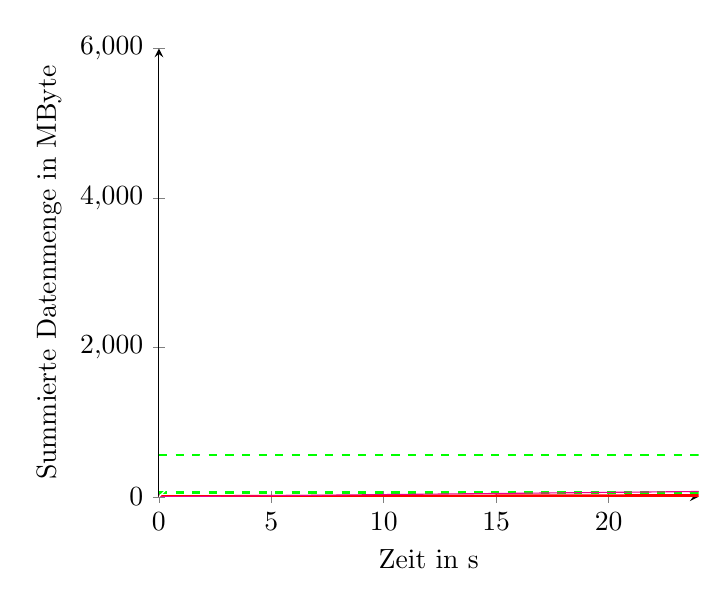
\begin{tikzpicture}
	\begin{axis} [domain=0:24, xlabel={Zeit in s}, ylabel={Summierte Datenmenge in $ \mathrm{MByte} $}, axis x line=bottom, axis y line=left, ymin=0, ymax=6000, xmin=0, xmax=24]
		\draw[blue, dashed] (100, 0) -- (100, 600);
		\node[blue, left, dotted] at (100, 590) (S1) {Videostart};
		\draw[blue, dashed] (200, 0) -- (200, 600);
		\node[blue, right, dotted] at (200, 590) (S2) {Videoende};
		\draw[blue, dashed] (190, 400) -- (190, 600);
		\draw[->] (200, 400) -- node[below] {$ 1\,\mathrm{s} $}(190,400);
		\draw[green, dashed, thick] (0, 57.77) -- (240, 57.77);	
		\node[above, green] at (50, 57.77) {Datenmenge bei Videostart};
		\draw[green, dashed, thick] (0, 564.2) -- (240, 564.2);	
		\node[below, green] at (50, 564.2) {Gesamte Datenmenge};
		\draw[red, very thick] (0,0) -- (100, 57.77);
		\draw[red, very thick] (100, 57.77) -- (190, 564.2);
		\node[red, right, text width=3cm] at (150, 300){Minimum Datenübertragung};
		\draw[magenta] (0,0) -- node[left, text width=3cm] {Durchschnittliche Datenübertragung} (190, 564.2);{Minimum Datenübertragung}
		\addplot[white] expression {564.2/190 * x * 100};
		\node[right]  (K1) at (130, 100) {1. kritischer Punkt};
		\draw[->] (K1) -- (105, 60);
		\node[left]  (K2) at (165, 550) {2. kritischer Punkt};
		\draw[->] (K2) -- (185, 560);
	\end{axis}
\end{tikzpicture}